\documentclass[letterpaper,10pt]{article}

\usepackage{enumitem}
\usepackage{titling}
\usepackage{listings,listings-rust}
\usepackage{url}
\usepackage{soul}
\usepackage{hyperref}
\usepackage{setspace}
\usepackage{subfig}
\usepackage{sectsty}
\usepackage{pdfpages}
\usepackage{colortbl}
\usepackage{multirow}
\usepackage{multicol}
\usepackage{relsize}
\usepackage{amsmath}
\usepackage{wasysym}
\usepackage{fancyvrb}
\usepackage[yyyymmdd]{datetime}
\usepackage{amsmath,amssymb,amsthm,graphicx,xspace}
\usepackage[titlenotnumbered,noend,noline]{algorithm2e}
\usepackage[compact]{titlesec}
\usepackage{XCharter}
\usepackage[T1]{fontenc}
\usepackage[scaled]{beramono}
\usepackage[normalem]{ulem}
\usepackage{booktabs}
\usepackage{tikz}
\usetikzlibrary{arrows.meta,automata,shapes,trees,matrix,chains,scopes,positioning,calc,decorations.pathreplacing}
\tikzstyle{block} = [rectangle, draw, fill=blue!20, 
    text width=2.5em, text centered, rounded corners, minimum height=2em]
\tikzstyle{bw} = [rectangle, draw, fill=blue!20, 
    text width=4em, text centered, rounded corners, minimum height=2em]

\definecolor{namerow}{cmyk}{.40,.40,.40,.40}
\definecolor{namecol}{cmyk}{.40,.40,.40,.40}
\renewcommand{\dateseparator}{-}

\let\LaTeXtitle\title
\renewcommand{\title}[1]{\LaTeXtitle{\textsf{#1}}}

\lstset{basicstyle=\footnotesize\ttfamily,breaklines=true}

\newcommand{\CPP}{C\nolinebreak\hspace{-.05em}\raisebox{.4ex}{\tiny\bf +}\nolinebreak\hspace{-.10em}\raisebox{.4ex}{\tiny\bf +}}
\def\CPP{{C\nolinebreak[4]\hspace{-.05em}\raisebox{.4ex}{\tiny\bf ++}}}

\newcommand{\handout}[5]{
  \noindent
  \begin{center}
  \framebox{
    \vbox{
      \hbox to 5.78in { {\bf ECE459: Programming for Performance } \hfill #2 }
      \vspace{4mm}
      \hbox to 5.78in { {\Large \hfill #4  \hfill} }
      \vspace{2mm}
      \hbox to 5.78in { {\em #3 \hfill \today} }
    }
  }
  \end{center}
  \vspace*{4mm}
}

\newcommand{\lecture}[3]{\handout{#1}{#2}{#3}{Lecture #1}}
\newcommand{\tuple}[1]{\ensuremath{\left\langle #1 \right\rangle}\xspace}

\addtolength{\oddsidemargin}{-1.000in}
\addtolength{\evensidemargin}{-0.500in}
\addtolength{\textwidth}{2.0in}
\addtolength{\topmargin}{-1.000in}
\addtolength{\textheight}{1.75in}
\addtolength{\parskip}{\baselineskip}
\setlength{\parindent}{0in}
\renewcommand{\baselinestretch}{1.5}
\newcommand{\term}{Winter 2021}

\singlespace


\begin{document}

\lecture{22 --- GPU Programming (CUDA) }{\term}{Jeff Zarnett, based on original by Patrick Lam}

\section*{GPUs: Heterogeneous Programming}

The next part will be about programming for heterogeneous
architectures. In particular, we'll talk about GPU programming, as
seen in CUDA. The general idea is to
leverage vector programming; vendors use the term SIMT (Single
Instruction Multiple Thread) to describe this kind of
programming. We've talked about the existence of SIMD instructions
previously, but now we'll talk about leveraging SIMT more
consciously. We are again in the domain of embarrassingly parallel
problems.

\paragraph{Cell, CUDA, and OpenCL.} 
Other examples of heterogeneous programming include
programming for the PlayStation 3 Cell~\cite{cellprimer} architecture and CUDA. (Note that the PS4 returns to a regular CPU/GPU configuration; however, it uses AMD hardware which combines the CPU and GPU on one chip.) The Cell includes a PowerPC core as well as
8 SIMD coprocessors:

\begin{center}
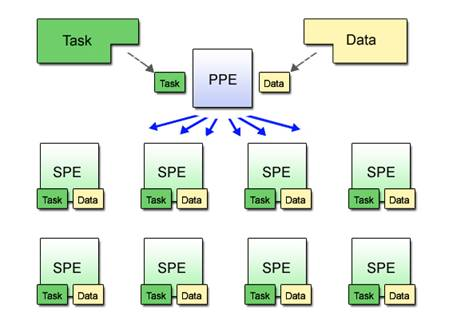
\includegraphics[width=.4\textwidth]{images/cell.jpg}
\end{center}
\hfill (from the Linux Cell documentation)

CUDA (Compute Unified Device Architecture) is NVIDIA's architecture
for processing on GPUs. ``C for CUDA'' predates OpenCL; NVIDIA still
makes CUDA tools available, and they may be faster than OpenCL on NVIDIA
hardware. On recent devices, you can use (most) \CPP~features in CUDA code,
which you can't do in OpenCL code. We used to teach OpenCL, but it seems
to be the case that CUDA has found widespread acceptance out in industry.
Hence, we use CUDA in the course. If you really need cross-platform or 
you have AMD hardware, then you want OpenCL. The principles are similar 
enough that you can take what you learned in one toolchain and apply it 
to the other.

\paragraph{Programming Model.} The programming
model for all of these architectures is similar: you write the code for
the massively parallel computation (kernel) separately from the main
code. Then at run-time, set up the data (input), transfer the data to the GPU, wait while the GPU executes the kernel, then transfer the results back. 

It makes sense to hand it over to the GPU because there are a lot of cores, although they run at a slower speed when compared to the CPU. Looking at the hardware in the ECE servers as of Fall 2020, ecetesla2 has a 4 core 3.6 GHz CPU. It also has 1920 CUDA cores that run at about 1.8 GHz. So, half the speed, but 480 times the workers. Sounds like we could get quite some speedup... if the workload is suitable.

At run-time, there is significant set-up cost for interacting with the GPU and then the data transfers (input to the GPU and collecting the results) mean there is a significant overhead cost for using the GPU. But the GPU can do lots of work in parallel once it gets going. This is a lot like deciding whether to drive or fly. 

If the distance is short, say, 200 km (the distance between Ottawa and Montreal) then flying makes no sense: you have to get to the airport, be there at least an hour or two early to make your way through security checkpoints, then fly, then get from the destination airport to your final destination. Sure, the flying part is fast, but the overhead makes your total average speed not worth it.

On the other hand, if you're going a longer distance, like 4000 km (roughly the distance between Waterloo and San Francisco), then driving is way slower! Sure, the overhead of going the airport remains, but once you're in the air you're moving at 800 km/h or so and in 5.5 hours you are there. Compare that to 40 hours of driving.

CUDA includes both task parallelism and data parallelism, as we've
discussed earlier in this course. \emph{Data parallelism} is the central
feature. You are evaluating a function, or \emph{kernel},
at a set of points. Each point represents a data element, such as one of the
bodies in the n-body simulation. But you could also perform some 
transformation on each pixel of an image or each frame of a video. If you 
imagine a 2-dimensional problem, each little circle in the diagram below is
a work-item:

\begin{center}

\begin{tikzpicture}
\foreach \x in {0,0.25,...,2}
  \foreach \y in {0,0.25,...,2}
    \draw (\x, \y) circle (0.25mm);
\end{tikzpicture}
\end{center}

Another name for the set of points is the \emph{index space}. 
Each of the points corresponds to a \emph{work-item}.

CUDA also supports \emph{task parallelism}: it can run different
kernels in parallel. Such kernels may have a one-point index space. This is
doing a large number of different things in parallel. We're not really going
to focus on that and will instead stick to the part about data parallelism.

\paragraph{More on work-items.} The work-item is the fundamental
unit of work. These work-items live on an $n$-dimensional
grid (ND-Range); we've seen a 2-dimensional grid above. You may choose
to divide the ND-Range into smaller work-groups, or the system can
divide the range for you. CUDA spawns a thread for each work item,
with a unique thread ID; they are grouped into blocks. Blocks can share 
memory locally, but each block has to be able to execute independently.
That is, the system can schedule the blocks to run in any order and possibly
in parallel (we hope so!). 

You get your choice about block size. Usually, we say let the system decide. However, for some computations it's better to specify; if you do, however, you want to make best use of the hardware and use a multiple of the size of the \textit{warp}. A warp is the NVIDIA term for a unit of execution, and there can be multiple units of execution in a given GPU.

\paragraph{Shared memory.} CUDA makes lots of different types of
memory available to you:

\begin{itemize}
\item private memory: available to a single work-item;
\item local memory (aka ``shared memory''): shared between work-items
  belonging to the same work-group; like a user-managed cache;
\item global memory: shared between all work-items as well as the host;
\item constant memory: resides on the GPU, and cached. Does not change.
\item texture memory: this is global memory too, also cached, and it provides potentially a very slight speedup over using global memory. The GPU has texture memory and caches that it uses for rendering and interpolating textures, and it's available for the GPU's general-purpose operations if your use case is a match. 
\end{itemize}

Choosing which kind of memory to use is an important design decision. A simple kernel might put everything in global memory, but that's likely to be slower than making good use of local memory. It could also be tempting to put all unchanging data in the constant memory, but its space is limited, so giant vectors won't always fit.

There is also host memory (RAM in your computer), which generally contains the application's data. We will be doing explicit transfers of the data from host memory to the GPU memory, in both directions.

\paragraph{My very own Kernel.} Let's start looking at a kernel. This is the code that will be executed by every CUDA thread somewhat in parallel. First, let's see what the code would look like if we just wrote it in \CPP:

\begin{lstlisting}[language=C++]
void vector_add(int n, const float *a, const float *b, float *c) {
  for (int i = 0; i < n; i++) {
    c[i] = a[i] + b[i];
}
\end{lstlisting}


The same code looks like this as a kernel~\cite{cuda}:
\begin{lstlisting}[language=C++]
__global__ void vector_add(float* A, float* B, float* C)
{
    int i = threadIdx.x;
    C[i] = A[i] + B[i];
}
\end{lstlisting}

We can see in this example that there's no more loop. This is because the loop has become implicit. The loop induction variable here is something we retrieve from \texttt{threadIdx.x} --- the thread index. The index is a three-component vector so it has x, y, and z dimensions. For this one-dimensional (linear) problem, we only need the first component (x). We'll come back to multi-dimensional problems later.

You can write kernels in a variant of \CPP, and it looks mostly like the language we (hopefully) know, with a few additions like the \texttt{\_\_global\_\_} designation in the previous example. A large number of features of more recent versions of the language are supported, but how much will vary based on your release of the kernel compiler (\texttt{nvcc}). There's a list of things that are not allowed in device code. It's unlikely that we'll be doing too many things that are exotic enough to be forbidden by the compiler, in this course. However, if you aren't sure why something isn't working or want to know what kind of stuff is not allowed, see \url{https://docs.nvidia.com/cuda/cuda-c-programming-guide/index.html#restrictions}. We might mention some restrictions if we encounter any in thing to write example kernels.

The kernel itself is compiled into a form called PTX -- Parallel Thread eXecution -- instructions. It's possible to write those directly, but we won't; we'll just let the compiler do it. In theory, as with assembly instructions, it might be possible for an expert to produce better PTX instructions than the compiler does, but let's assume we're not. Also, using the \texttt{nvcc} compiler makes it so your kernel will run on whatever hardware you have. Just as you would when compiling in another language, it's advised to recompile if you change machines (e.g., uploading to ECE servers from your laptop, or switching from one ECE server to another).

The \texttt{nvcc} compiler has specific requirements for the underlying compiler it relies. For example, on \texttt{ecetesla2} at the time of writing, \texttt{nvcc} fails without specifying \texttt{gcc} version 6 instead of the default. With the command \texttt{nvcc --compiler-bindir /usr/bin/gcc-6 -ptx nbody.cu}, it will compile. 

Remember that the kernel has none of the safety guarantees that we normally get in Rust! We can easily read off the end of an array, forget to initialize a variable, allocate memory that we forget to deallocate, or have race conditions, amongst other things. So not only can you encounter runtime errors in your kernel, but also that it's wise to check that your output matches expectations rather than just assume it's fine. So, just because it compiles, doesn't mean it will work.

If you want a quick example of what can go wrong with the kernel at runtime, here's something I got in testing:
{\scriptsize
\begin{verbatim}
thread 'main' panicked at 'Failed to deallocate CUDA Device memory.: IllegalAddress', 
/home/jzarnett/.cargo/registry/src/github.com-1ecc6299db9ec823/rustacuda-0.1.2/src/memory/device/device_buffer.rs:259:32
note: run with `RUST_BACKTRACE=1` environment variable to display a backtrace
thread 'main' panicked at 'Failed to deallocate CUDA Device memory.: IllegalAddress', 
/home/jzarnett/.cargo/registry/src/github.com-1ecc6299db9ec823/rustacuda-0.1.2/src/memory/device/device_buffer.rs:259:32
stack backtrace:
\end{verbatim}
}

\paragraph{More complex kernel example.} Here's a kernel we wrote for the N-body problem that we saw earlier. It is the version without the approximations optimization; just the straightforward brute-force approach: 

\begin{lstlisting}[language=C++]
__device__ void body_body_interaction(float4 point1, float4 point2, float3 *acceleration) {
    float4 difference;

    difference.x = point2.x - point1.x;
    difference.y = point2.y - point1.y;
    difference.z = point2.z - point1.z;
    difference.w = 1.0f;

    float distSqr = difference.x * difference.x + difference.y * difference.y + difference.z * difference.z + 1e-10;

    float distSixth = distSqr * distSqr * distSqr;
    float invDistCube = 1.0f / sqrtf(distSixth);

    float s = point2.w * invDistCube;

    acceleration->x += difference.x * s;
    acceleration->y += difference.y * s;
    acceleration->z += difference.z * s;
}

extern "C" __global__ void calculate_forces(const float4* positions, float3* accelerations, int num_points) {
    if (blockIdx.x >= num_points) {
        return;
    }
    float4 current = positions[blockIdx.x];
    float3 acc = accelerations[blockIdx.x];

    for (int i = 0; i < num_points; i++) {
        body_body_interaction(current, positions[i], &acc);
    }
    accelerations[blockIdx.x] = acc;
}
\end{lstlisting}

Let's break it down. The calculation of forces between bodies takes some \texttt{float4} and \texttt{float3} arguments. In the Rust example, I made my own \texttt{Point} and \texttt{Acceleration} types. CUDA uses \textit{vector types}, which are a group of $n$ of that primitive type. So a \texttt{float4} is a grouping of four \texttt{float}s where the components are referred to as \texttt{x, y, z, w}. There exist vector types for the standard C primitives (e.g., \texttt{int, uint, float, double, char}, and some more) in sizes of 1 through 4. It's just a nice way to package up related values without needing a custom structure (although you can send structures in to kernels). When we get to the host code you'll see that I've had to modify its representation of the data as well.

The function also is prefixed with \texttt{\_\_device\_\_} which indicates that it will be called from another function when running on the GPU. A \texttt{\_\_global\_\_} function (as the calculation of forces is called from the host, and such global functions can call device functions but not other global functions. Device functions can call only other device functions. So it makes it clear where the entry points are from host code. In some OOP-sense, you could consider the device functions to be ``private'', not that I encourage you to think that way.

The only other thing that really stands out is the \texttt{extern "C"} declaration at the beginning of the global function. This disables what is called \textit{name mangling} or \textit{name decoration}, which is to say a compiler trying to differentiate between multiple functions with the same name. If this is too compiler-magic to worry about, just place this magic spell in front of the function call and it prevents the compiler from telling you it can't find the function by the name you specified. More modern versions of \texttt{nvcc} may not have this problem, mind you.

We'll also be using the N-body kernel soon as an example for when we examine how to launch a CUDA program. Also, if you're curious, the compiled version of the kernel resembles assembly language. The output is a little too large to show in the notes/slides, but the compiled version is in the course repository.

\subsection*{Writing a Kernel Well}

To start with, of course, we need to decide what sort of work belongs in the kernel to begin with. Anything that would benefit from the very large number of execution units is a good candidate, so that's typically things that are the iterations of a loop. If the loops need to be sequential, though, this is not a good use of the parallelism. If you need a little bit of coordination, we can achieve that, though, with barriers (similar to the concept as seen in concurrency). 

Comparing the first kernel that we saw against its CPU-code equivalent, we've taken the explicit for loop and made it implicit as a one-dimensional problem. We just use the GPU on the outer loop. What if we wanted to make it a two-dimensional problem? We could instead treat each pair of points $(i, j)$ as a point in the space, making it a two-dimensional problem. Then you could think of it as a matrix rather than an array and provide it to CUDA like that. This might increase the parallelism! 

Although that sounds good, for the N-body problem, it's not. The calculation of body-body interaction for just one pair of points is a very small amount of work, tiny even. Having one work-item for each such calculation means there's a lot of overhead to complete the calculation and it doesn't make sense. But if the calculation of the interaction were more complex, then this transformation might be an improvement.

We can also have three-dimensional problems. If you want something more than a three-dimensional, you have to have some loops in your code. So that 6-level-deep nested-for-loop? You can have the outer three loops as your x, y, and z dimensions, but the rest will be in for loops. Can't avoid everything, I am afraid. The limit to three dimensions is probably because graphics cards were designed for rendering images in 3-D so it seems logical? But that's only a guess.

Of course, you can sometimes flatten the dimensions of your problem a bit. A rectangular array in C/\CPP~is really stored as a linear array and the \texttt{[x][y]} is just notational convenience so you could easily just treat it as a linear array. If that's the case, you can avoid the need for a loop in your code. In the N-Body problem, having more items of smaller size is not an improvement because they're too small to be meaningful. Maybe a different problem would have different characteristics.

Consider something like brute-forcing a password of 6 characters (easy, but just for the purpose of an example). A one-dimensional approach might generate (in host code) one starting possibility for each valid character in the first position and then let the kernel loop over all possible other values. Then you might be able to improve that by generating starting possibilities in a 3-D matrix for the first three positions and loop in the kernel after that. Whether this is better or not is something that needs testing. And then one could think about generating more starting possibilities by flattening another dimension. It might be faster if it allows more things to be checked in parallel, but it might be slower because of the extra time spent generating the initial conditions in the host code. And eventually at some point (when there are longer passwords), there are too many possibilities to reasonably fit in the host code memory and it becomes impractical to transfer them to and from the GPU.

Of course, this isn't necessarily the best way to brute-force a password. We'll return to that subject later!

\paragraph{Branches.} CUDA implements a SIMT architecture. The documentation warns you, however, that unlike a CPU, there's neither branch prediction nor speculative execution. This means that branches are much more costly than they would be on the CPU. 

In practice, the hardware will execute all branches that any thread in
a warp executed (which can be slow). It then keeps only the results that are valid. Consider this brief example:

    \begin{verbatim}
__global__ void contains_branch(float *a, float *b) {
    if (condition()) {
        a[blockIdx.x] += 5.0;
    } else {
        b[blockIdx.x] += 5.0;
    }
}
\end{verbatim}

In the above example, the {\tt if} statement will cause
the warp both branches of the {\tt if}, keeping only the
result that is correct. But still, unnecessary work is done. It won't be possible to avoid all conditional branches, but they get expensive quickly.

Similarly, executing a loop will cause the
workgroup to wait for the maximum number of iterations of the loop in
any work-item. The compiler will try to unroll loops if they have a known number of iterations. Here, an example from the CUDA docs of a loop it can unroll:

{\scriptsize \hspace*{2em} \begin{minipage}{.5\textwidth}
    \begin{lstlisting}
__device__ void foo(int *p1, int *p2) {
  for (int i = 0; i < 12; ++i) {
    p1[i] += p2[i]*2;
  }
}
    \end{lstlisting}
\end{minipage} }

\paragraph{Atomic functions.}

We also mentioned earlier that there's still the possibility of race conditions. This means that if you want to, say, concurrently add to the same location, you need to use atomic functions. The atomic operations are usable on the standard primitive types like integers, floating point numbers, etc. And there are atomic operations for adding, subtracting, min, increment, decrement, as well as compare-and-swap and bitwise operations. Here's a quick example from the docs on a compare-and-swap~\cite{cuda}:

\begin{lstlisting}[language=C++]
__device__ double atomicAdd(double* address, double val) {
    unsigned long long int* address_as_ull =
                              (unsigned long long int*)address;
    unsigned long long int old = *address_as_ull, assumed;

    do {
        assumed = old;
        old = atomicCAS(address_as_ull, assumed,
                        __double_as_longlong(val +
                               __longlong_as_double(assumed)));

    // Note: uses integer comparison to avoid hang in case of NaN (since NaN != NaN)
    } while (assumed != old);

    return __longlong_as_double(old);
}
\end{lstlisting}

\subsection*{Launch?}

So far, all we have covered is the theory and then how to write a kernel. To make use of it, we'll have to look at the host code. That's our next topic. 


\bibliographystyle{alphaurl}
\bibliography{459}


\end{document}
